\documentclass[10pt,a4paper,float]{article}
\usepackage[utf8]{inputenc}
\usepackage[czech]{babel}
\usepackage{amsmath}
\usepackage{amsfonts}
\usepackage{amssymb}
\usepackage{bm}
\usepackage{graphicx}
\usepackage{lmodern}
\usepackage{float}
\usepackage{hyperref}
\usepackage{icomma}
\usepackage{parskip}
\usepackage[left=2cm,right=2cm,top=2cm,bottom=2cm]{geometry}
\setlength{\parindent}{0pt}
\author{Šťur}
\title{Použití TI-89 v úlohách předmětu BPC-MA3}
\begin{document}
\maketitle

\pagebreak

\tableofcontents

\pagebreak

\section{Prerekvizity}
\label{sec:pre}
Vyžadován je tabulkový editor CellSheet, který si můžete stáhnout zde:\\ \url{https://education.ti.com/en/software/details/en/C348D29C99284143B9E3FE93CF6742A6/89cellsheet}

Taktéž je vyžadován Simultaneous Equation Solver App for the TI-89 Titanium, ke stažení zde:\\ \url{https://education.ti.com/en/software/details/en/BD358C4836B84DBCBA254D6554FBBEAC/89simultaneousequationsolver}

\section{Základní práce s kalkulačkou}
\label{sec:zaklady}
\subsection{Změna aktuálně používané složky a její vytvoření}
\label{ssec:slozky}
Je praktické si vytvářet pro různé předměty složky a práci soustředit do nich.

Vytvoření probíhá následovně:

Klávesovou kombinací [2nd]+[-] vyvoláme VAR-LINK menu.

Klávesou [F1] následně vyvoláme Manage menu, Create folder je pátá položka.

\begin{figure}[H]
	\centering
	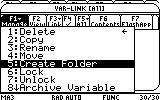
\includegraphics[width=.5\textwidth]{img/CREATEFOLDER}
\end{figure}

Pomocí [ESC] obrazovku opustíme.

Chceme-li se do složky přepnout, vyvoláme klávesou [MODE] nastavení kalkulačky a změníme druhou položku.

\begin{figure}[H]
	\centering
	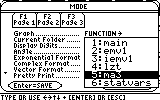
\includegraphics[width=.5\textwidth]{img/CHANGEFOLDER}
\end{figure}

Položku volíme šipkou doprava, potvrzujeme klávesou [ENTER] a s uložením nastavení opouštíme taktéž klávesou [ENTER].

\textit{Poznámka: pro účely počítání MA3 může být praktické vynucení zobrazování výsledků jako desetinných čísel. V MODE menu se klávesou [F2] přepněte na stranu 2 a Exact/Approx položku změňte na APPROXIMATE a uložte.}

\pagebreak

\subsection{Uložení funkce jedné proměnné}
\label{ssec:ulozeni1fce}
V MODE menu se ujistěte, že položka Graph je nastavena na FUNCTION.

Klávesovou kombinací [$\diamond$]+[F1] vyvoláme Y= menu. Zde můžeme do jednotlivých proměnných ukládat kýžené funkce.

\begin{figure}[H]
	\centering
	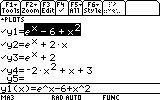
\includegraphics[width=.5\textwidth]{img/1FUNC}
\end{figure}

Uložit funkci do funkční proměnné lze taktéž z výchozí obrazovky následovně. Šipka je vyvolána klávesou [STO~$\triangleright$].

\begin{figure}[H]
	\centering
	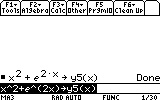
\includegraphics[width=.5\textwidth]{img/1FUNC_ULOZ}
\end{figure}

Obecně v TI-89 ukládáme výsledky již při zadávání příkladu pomocí [STO $\triangleright$] a kýženého názvu proměnné, který u běžných číselných/maticových/řetězcových výsledků může být jakýkoliv (např. mnouk).

Ve výpočtech pak tyto funkce můžeme využívat následovně:

\begin{figure}[H]
	\centering
	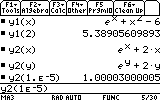
\includegraphics[width=.5\textwidth]{img/1FUNC_UZITI}
\end{figure}

Pakliže výsledek není ve tvaru, který by nám vyhovoval (například je zlomkem), jako desetinné číslo ho můžeme zobrazit, pakliže místo klávesy [ENTER] použijeme kombinaci [$\diamond$]+[ENTER] ($\approx$).

\pagebreak

\subsection{Uložení funkce dvou proměnných}
\label{ssec:ulozeni2fce}
V MODE menu je nutno položku Graph přepnout do 3D:

\begin{figure}[H]
	\centering
	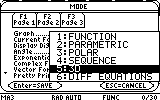
\includegraphics[width=.5\textwidth]{img/3D}
\end{figure}

Práce pak probíhá stejně, jako s funkcí jedné proměnné:

\begin{figure}[H]
	\centering
	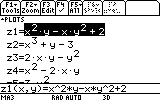
\includegraphics[width=.5\textwidth]{img/2FUNC}
\end{figure}

Musíme však mít na paměti, že do závorek za názvem proměnné je třeba dosadit 2 hodnoty, jelikož jde o funkci dvou proměnných:

\begin{figure}[H]
	\centering
	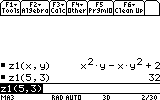
\includegraphics[width=.5\textwidth]{img/2FUNC_UZITI}
\end{figure}

\pagebreak

\subsection{Vytvoření matice/vektoru}
\label{ssec:matice}
Velmi jednoduché matice můžeme zadat přímo z výchozí obrazovky, je to však praktické nanejvýš u vektorů. Vektor [5;3] zadáme jako:

[[5][3]]

Pro větší matice je žádoucí používat vestavěnou aplikaci Data/Matrix Editor, kterou nalezneme v APPS nabídce. Zvolíme New, což nás dostane na následující obrazovku:

\begin{figure}[H]
	\centering
	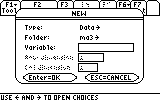
\includegraphics[width=.5\textwidth]{img/DATAEDITOR}
\end{figure}

Type je nutno přepnout na Matrix, do kolonky Variable zadáme název proměnné, do Row dimension a Col dimension pak počet řádků, respektive sloupců.
Na následujícím obrázku je příklad vytvoření 2x2 matice s názvem "mnau":

\begin{figure}[H]
	\centering
	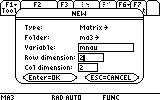
\includegraphics[width=.5\textwidth]{img/MNAUMATRIX}
\end{figure}

Po potvrzení můžeme zadávat:

\begin{figure}[H]
	\centering
	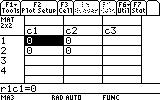
\includegraphics[width=.5\textwidth]{img/MATRIXEDIT1}
\end{figure}

\pagebreak

Kromě čísel je možno do matice vkládat i funkce:
\begin{figure}[H]
	\centering
	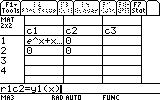
\includegraphics[width=.5\textwidth]{img/MATRIXEDIT2}
\end{figure}

Aplikaci opustíme QUIT kombinací, ([2ND]+[ESC]), uložení je automatické.

Na výchozí obrazovce pak matici vyvoláme prostým zadáním názvu proměnné, můžeme s ní i provádět libovolné dovolené matematické operace:

\begin{figure}[H]
	\centering
	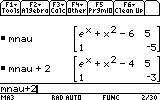
\includegraphics[width=.5\textwidth]{img/UZITIMATIC1}
\end{figure}

V matici máme dosazenou funkci. Pakliže chceme za proměnné ve funkci (nejen u matic) dynamicky dosazovat, použijeme za příkladem (a před případným STO) $\vert$x=(číslo). Svislou čáru vyvoláme klávesou [ $\vert$ ].

\begin{figure}[H]
	\centering
	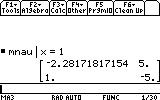
\includegraphics[width=.5\textwidth]{img/UZITIMATIC2}
\end{figure}

\pagebreak

U funkcí více proměnných používáme $\vert$x=(číslo) and y=(číslo). Je nutno to napsat i s mezerami, pro usnadnění si jde " and " i s mezerami najít v nabídce CATALOG vyvolané tlačítkem [CATALOG]. V CATALOGu je možno se rychle pohybovat pomocí počátečního písmena, která můžeme vidět u jednotlivých kláves bíle. Pro přeskok do sekce funkcí začínajících písmenem 'a' stiskneme klávesu [=]:

\begin{figure}[H]
	\centering
	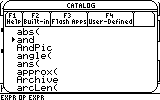
\includegraphics[width=.5\textwidth]{img/CATALOG}
\end{figure}

Výsledek pro funkci dvou proměnných je takovýhle:

\begin{figure}[H]
	\centering
	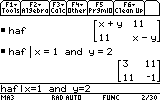
\includegraphics[width=.5\textwidth]{img/UZITIMATIC3}
\end{figure}

\subsection{Derivování}
\label{ssec:derivace}
Derivovat můžeme přímo z výchozí obrazovky, potřebnou funkci vyvoláme kombinací [2ND]+[8]. První parametr je vstupní funkce, druhý proměnná, podle které derivujeme (díky tomu je možno provádět i parciální derivace). Vstupem může být jak ručně napsaná funkce, tak funkce uložená do speciální proměnné:

\begin{figure}[H]
	\centering
	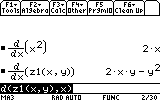
\includegraphics[width=.5\textwidth]{img/DERIVACE}
\end{figure}

\pagebreak

\subsection{Integrování}
\label{ssec:integrace}
Integrovat můžeme přímo z výchozí obrazovky, potřebnou funkci vyvoláme kombinací [2ND]+[7]. Funkce má 4 parametry, 2 jsou volitelné. První parametr je vstupní funkce, druhý proměnná, podle které integrujeme. Vstupem může být jak ručně napsaná funkce, tak funkce uložená do speciální proměnné:

\begin{figure}[H]
	\centering
	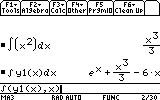
\includegraphics[width=.5\textwidth]{img/INTEGROVANI1}
\end{figure}

Pakliže chceme použít určitý integrál, využijeme i třetí a čtvrtý parametr, kterým je dolní a horní mez:

\begin{figure}[H]
	\centering
	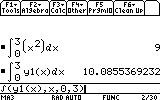
\includegraphics[width=.5\textwidth]{img/INTEGROVANI2}
\end{figure}

\subsection{Základy práce s tabulkovým procesorem CellSheet}
\label{ssec:cellsheet}
Aplikaci CellSheet, pakliže ji máme nainstalovanou, vyvoláme z nabídky APPS -> FlashApps... -> CellSheet, kde z nabídky zvolíme New. V dialogu zvolíme složku a název proměnné. Otevře se nám okno nápadně připomínající Excel:

\begin{figure}[H]
	\centering
	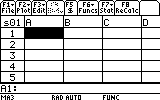
\includegraphics[width=.5\textwidth]{img/CELL1}
\end{figure}

Práce probíhá téměř na chlup stejně jako se známým tabulkovým procesorem. Vzorce začínáme rovnítkem, buňky označujeme kombinací sloupec+řádek (např. A1, možno psát i a1), konstantní řádky/sloupce/buňky ve vzorci označujeme dolarem pomocí klávesy [F5].

\pagebreak

Pakliže zvolená funkce (např. sum) pracuje s rozsahem buněk, oddělíme ve vzorci buňky dvojtečkou, např. =sum(a1:a3):

\begin{figure}[H]
	\centering
	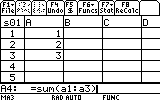
\includegraphics[width=.5\textwidth]{img/CELL2}
\end{figure}

Po vzoru konvenčních tabulkových procesorů je taktéž možno vybranou buňku s nějakým vzorcem zkopírovat (pomocí kombinace [$\diamond$]+[ $\uparrow$ ], vybrat rozsah buněk, kam chceme vzorec vložit (za stálého stisku klávesy [ $\uparrow$ ] mačkáme šipku odpovídající kýženému směru, dokud není zvolen žádaný rozsah)...

\begin{figure}[H]
	\centering
	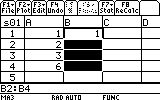
\includegraphics[width=.5\textwidth]{img/CELL3}
\end{figure}

...načež pomocí [$\diamond$]+[ESC] provedeme vložení:

\begin{figure}[H]
	\centering
	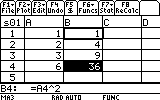
\includegraphics[width=.5\textwidth]{img/CELL4}
\end{figure}

Chceme-li hodnotu nějaké buňky exportovat do standardní proměnné, vybereme v Edit ([F3]) nabídce funkci Export...

\pagebreak

V dialogu zvolíme Type: Expr, do Variable vložíme název proměnné, do Cell zadáme buňku (bývá předvyplněno, pakliže jsme export vyvolali na námi kýžené buňce) a odentrujeme.

\begin{figure}[H]
	\centering
	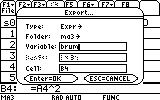
\includegraphics[width=.5\textwidth]{img/CELL5}
\end{figure}

\subsection{Řešení soustav lineárních rovnic}
\label{ssec:linsoustavy}
Stejně jako u Casio kalkulaček lze toto řešit pomocí matic, což však může být zdlouhavé. Lze si nicméně nainstalovat aplikaci Simultaneous Eqn Solver.

Tu spustíme pomocí APPS -> FlashApps... -> Simultaneous Eqn Solver. Z nabídky vybereme New...

Dialog se nás zeptá na počet rovnic a neznámých, který zadáme, například 2 a 2. Otevře se toto okno:

\begin{figure}[H]
	\centering
	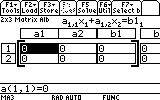
\includegraphics[width=.5\textwidth]{img/SYSEQ1}
\end{figure}

Zápis provádíme maticově, sloupce a1 až an označují matici neznámých, sloupec b1 je vektor pravé strany. Předpokládejme, že chceme vložit následující rovnici:

\begin{align*}
	x + y &= 5\\
	2x - 3y &= 2
\end{align*}

Zápis bude vypadat takto:

\begin{figure}[H]
	\centering
	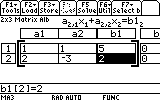
\includegraphics[width=.5\textwidth]{img/SYSEQ2}
\end{figure}

\pagebreak

Výsledky vyvoláme stisknutím klávesy [F5]:

\begin{figure}[H]
	\centering
	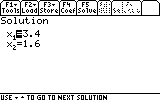
\includegraphics[width=.5\textwidth]{img/SYSEQ3}
\end{figure}

\pagebreak

\section{Numerické metody}
\label{sec:nummetody}
\subsection{Metoda nejmenších čtverců}
\label{ssec:ctverce}
Metodou nejmenších čtverců proložte následující body parabolou.

\begin{table}[H]
	\centering
	\begin{tabular}{l|l|l|l|l}
		x & 2,8 & 3,2 & 3,5 & 3,9 \\ \hline
		y & 0,4 & 0,3 & 0,8 & 1,1
	\end{tabular}
\end{table}

Tato úloha je ideální pro využití aplikací CellSheet a Simultaneous Equation Solver, s jejichž správným využitím lze minimalizovat možnost lidské chyby.

Soustava rovnic pro kvadratickou aproximaci metodou nejmenších čtverců je následující:

\begin{align*}
	C_0 (n + 1) + C_1 \sum_{i=0}^{n} x_i + C_2 \sum_{i=0}^{n} x_i^2 &= \sum_{i=0}^{n} y_i \\
	C_0 \sum_{i=0}^{n} x_i + C_1 \sum_{i=0}^{n} x_i^2 + C_2 \sum_{i=0}^{n} x_i^3 &= \sum_{i=0}^{n} x_i y_i \\
	C_0 \sum_{i=0}^{n} x_i^2 + C_1 \sum_{i=0}^{n} x_i^3 + C_2 \sum_{i=0}^{n} x_i^4 &= \sum_{i=0}^{n} x_i^2 y_i
\end{align*}

Ze soustavy je patrné, že potřebujeme vypočítat druhou, třetí a čtvrtou mocninu pro všechna $x$ v tabulce, součin $x$ a druhé mocniny $x$ s $y$ a provést součet všech sloupců vzniklé tabulky.

Vhodný layout je násldující:

\begin{table}[H]
	\centering
	\begin{tabular}{c|c|c|c|c|c|c|c}
		i & $x_i$ & $y_i$ & $x_i^2$ & $x_i^3$ & $x_i^4$ & $x_i y_i$ & $x_i^2 y_i$ \\ \hline
		\dots & \dots & \dots & \dots & \dots & \dots & \dots & \dots \\
		\dots & \dots & \dots & \dots & \dots & \dots & \dots & \dots \\ \hline
		$\sum$ & \dots & \dots & \dots & \dots & \dots & \dots & \dots \\
	\end{tabular}
\end{table}

Nyní si spustíme program CellSheet a vytvoříme novou tabulku. Do prvních dvou sloupců zadáme hodnoty x a y ze zadání:

\begin{figure}[H]
	\centering
	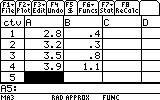
\includegraphics[width=.5\textwidth]{img/CTVERCE1.PNG}
\end{figure}

\pagebreak

Do buňky A5 nyní vložíme sumaci sloupce A, tedy hodnot $x_i$:\\
=sum(a1:a4)

\begin{figure}[H]
	\centering
	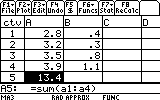
\includegraphics[width=.5\textwidth]{img/CTVERCE2.PNG}
\end{figure}

Abychom provedli i sumaci hodnot y, zkopírujeme buňku A5 do buňky B5. Klávesová kombinace pro kopírování je [$\diamond$]+[$\uparrow$], pro vložení [$\diamond$]+[ESC]. Pokud je buňka správně označena ke zkopírování, objeví se kolem ní tlustý rámeček.\\
\textit{Nápověda: povšimněte si žlutozelených nápisů COPY a PASTE nad dlačítky [$\uparrow$] a [ESC]. To značí, že pro jejich použití musíte stisknout žlutozelenou klávesu [$\diamond$]}

Po zkopírování je výsledek následovný:

\begin{figure}[H]
	\centering
	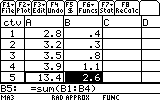
\includegraphics[width=.5\textwidth]{img/CTVERCE3.PNG}
\end{figure}

Do sloupce C můžeme vložit $x_i^2$. To provedeme vložením následujícího vzorce do buňky C1:\\
=a1$\land$2

Po jeho vložení buňku C1 zkopírujeme a kurzorem přejdeme do buňky níže. Stiskneme klávesu [$\uparrow$] a za jejího stálého držení přejdeme do buňky C4. Povšimněte si, že jsou všchny tyto buňky vybrány:

\begin{figure}[H]
	\centering
	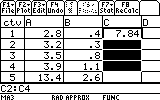
\includegraphics[width=.5\textwidth]{img/CTVERCE4.PNG}
\end{figure}

\pagebreak

Nyní stiskneme PASTE kombinaci ([$\diamond$]+[ESC]):

\begin{figure}[H]
	\centering
	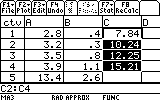
\includegraphics[width=.5\textwidth]{img/CTVERCE5.PNG}
\end{figure}

Ještě provedeme sumaci sloupce tím, že do buňky C5 zkopírujeme buňku B5:

\begin{figure}[H]
	\centering
	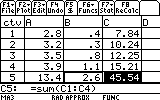
\includegraphics[width=.5\textwidth]{img/CTVERCE6.PNG}
\end{figure}

Pomocí těchto kroků vytvoříme i zbylé potřebné sloupce, jak je naznačeno na tabulce s layoutem:

\begin{figure}[H]
	\centering
	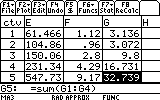
\includegraphics[width=.5\textwidth]{img/CTVERCE7.PNG}
\end{figure}

\pagebreak

Pakliže se chceme vyhnout lidské opisovací chybě, můžeme poněkud zdlouhavě vyexportovat potřebné hodnoty do proměnných. Ukážeme si to na buňce A5, tedy $\sum x_i$.

Kurzorem buňku vybereme, otevřeme nabídku Edit (klávesa [F3]) a otevřeme zde nabídku Export...

Jako Type zvolíme Expr (expression), zvolíme název (např. xi), ověříme, že je v kolonce Cell správná buňka a odenterujeme.

\begin{figure}[H]
	\centering
	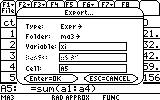
\includegraphics[width=.5\textwidth]{img/CTVERCE8.PNG}
\end{figure}

Tímto způsobem exportujeme všechny buňky se sumou.

Opustíme program CellSheet pomocí QUIT kombinace a spustíme program Simultaneous Eqn Solver. Počet rovnic je 3, počet proměnných taktéž.

\begin{figure}[H]
	\centering
	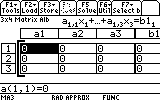
\includegraphics[width=.5\textwidth]{img/CTVERCE9.PNG}
\end{figure}

Do buňky a(1, 1) vložíme počet zadaných bodů, tedy 4. Do zbylých buňek vkládejte názvy proměnných odpovídající jednotlivým sumám. Všimnětě si, že se název proměnné po vložení změní na číslo.

Takto zadáme celou soustavu rovnic:

\begin{figure}[H]
	\centering
	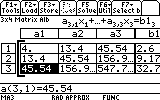
\includegraphics[width=.5\textwidth]{img/CTVERCE10.PNG}
\end{figure}

\pagebreak

Klávesou [F5] spustíme SOLVE a ukážou se nám výsledky:

\begin{figure}[H]
	\centering
	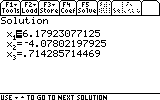
\includegraphics[width=.5\textwidth]{img/CTVERCE11.PNG}
\end{figure}

$x_1$ je $C_0$, $x_2$ je $C_1$ a $x_3$ je $C_2$, výsledná parabola je tedy:

\[
	y = 6,1792 - 4,0780 x + 0,7143 x^2
\]

\subsection{Řešení jedné nelineární rovnice Newtonovou metodou}
\label{ssec:1newton}
Je dána rovnice $e^x - 6 + x^2 = 0$.\\
Najděte interval délky 1 s celočíselnými mezemi, v němž leží záporný kořen této rovnice.

Prvně je potřeba nalézt interval žádané délky, v němž leží řešení. Toto je možno graficky, případně nalezením řešení pomocí solveru a určením intervalu z něj.

Solver je možno vyvolat pomocí funkce solve(), jejíž první argument je hledaná rovnice a druhý argument proměnná, která se v rovnici vyskytuje. Abychom nemuseli solve funkci psát manuálně, je možno ji vyvolat z Algebra menu skrývajícím se pod klávesou [F2]. Počítejte s možností, že kalkulačka může hledat řešení i půl minuty.

\begin{figure}[H]
	\centering
	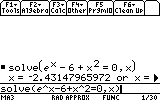
\includegraphics[width=.5\textwidth]{img/1NEWTON1.PNG}
\end{figure}

Záporný kořen je $x = -2,43$, interval tedy může být $<-3; -2>$.

\pagebreak

Pakliže jsme tak doteď neučinili, je záhodno si funkci uložit do Y= menu, viz kapitola \ref{ssec:ulozeni1fce}:

\begin{figure}[H]
	\centering
	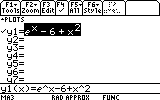
\includegraphics[width=.5\textwidth]{img/1NEWTON2.PNG}
\end{figure}

Nyní je potřebné funkci dvakrát zderivovat, pro návod vizte kapitolu \ref{ssec:derivace}.\\
\textit{Pozn.: Pro snadné uložení zderivované f-ce se kurzorem posuneme do výsledku, enterem ho přesuneme do vstupního řádku a nasměrujeme do proměnné y2(x), případně y3(x), viz kapitola \ref{ssec:ulozeni1fce}.}

\begin{figure}[H]
	\centering
	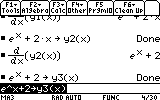
\includegraphics[width=.5\textwidth]{img/1NEWTON3.PNG}
\end{figure}

Nyní si vybereme jeden z krajních bodů nalezeného intervalu (zvolíme si $-3$) a ověříme konvergenci metody pomocí podmínky $f(x_0) \cdot f''(x_0) > 0$:

\begin{figure}[H]
	\centering
	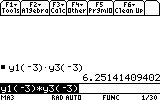
\includegraphics[width=.5\textwidth]{img/1NEWTON4.PNG}
\end{figure}

$6,25 > 0$, hodnotu $-3$ lze tedy použít jako počáteční aproximaci.

\pagebreak

Nyní si spustíme CellSheet a vytvoříme si novou tabulku. Do buňky A1 vložíme naši počáteční aproximaci.

\begin{figure}[H]
	\centering
	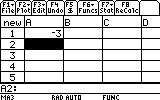
\includegraphics[width=.5\textwidth]{img/1NEWTON5.PNG}
\end{figure}

Další aproximaci lze zjistit z tohoto vzorce:
\[
	x_{k+1} = x_k - \frac{f(x_k)}{f'(x_k)}
\]

Funkci f(x) máme uloženou v y1(x), funkci f'(x) v y2(x), do buňky A2 pak tento vzorec vložíme následujícím způsobem:\\
=a1-y1(a1)/y2(a1)

Do buňky B2 vložíme přesnost výpočtu, kterou zjistíme ze vzorce:
\[
	\xi = |X_{k+1} - x_k|
\]
Což je možno vložit jako:\\
=abs(a2-a1)

Tímto jsme provedli 1 krok:

\begin{figure}[H]
	\centering
	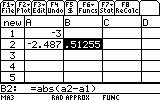
\includegraphics[width=.5\textwidth]{img/1NEWTON6.PNG}
\end{figure}

Nyní budeme postupně kopírovat hodnoty ze sloupce A a ze sloupce B níže, dokud nedosáhneme požadované přesnosti (například $10^{-3}$), kteréžto jsme dosáhli v buňce A4:


\begin{figure}[H]
	\centering
	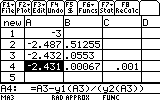
\includegraphics[width=.5\textwidth]{img/1NEWTON7.PNG}
\end{figure}

\textit{Pozn.: Šířka sloupce může být příliš malá na zobrazení hodnoty na dostatečný počet des. míst. Chceme-li sloupec rozšířit, tak při vybrané buňce z požadovaného sloupce zvolíme Edit -> Column Format, kde zvětšíme hodnotu Col Width (např. na 10) a Display Digit (např. na FLOAT 12)}.

\subsection{Řešení soustavy nelineárních rovnic Newtonovou metodou}

Je dána soustava rovnic

\begin{align*}
	x^2 y - x y^2 + 2 &= 0\\
	x^3 + y - 3 &= 0
\end{align*}

Řešte tuto soustavu Newtonovou metodou. Proveďte dva kroky metody. Vyjděte z bodu $ \left\{ x_0; y_0 \right\} = \left\{ 1; 1 \right\} $.

Nejprve je nutno kalkulačku přepnout do režimu práce s funkcemi dvou proměnných dle kapitoly \ref{ssec:ulozeni2fce}.

Funkce $f_1(x,y)$ a $f_2(x,y)$ uložíme do funkcí z1 a z2:

\begin{figure}[H]
	\centering
	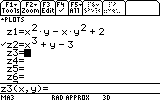
\includegraphics[width=.5\textwidth]{img/2NEWTON1.PNG}
\end{figure}

Následně v souladu s kapitolou \ref{ssec:derivace} vypočteme parciální derivace obou funkcí (tj. vypočteme derivaci obou funkcí podle x a podle y) a v souladu s kapitolou \ref{ssec:ulozeni2fce} (podrobněji v kapitle \ref{ssec:ulozeni1fce}) je uložíme do proměnných:

\begin{figure}[H]
	\centering
	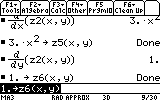
\includegraphics[width=.5\textwidth]{img/2NEWTON2.PNG}
\end{figure}

Počítejme s následujícím uložením: $\frac{\partial f_1}{\partial x}$ = z3, $\frac{\partial f_1}{\partial y}$ = z4, $\frac{\partial f_2}{\partial x}$ = z5, $\frac{\partial f_2}{\partial y}$ = z6

\pagebreak

Následná aproximace pro soustavy nelineárních rovnic se počítá dle následujících vzorců:
\[
	\mathbf{F'}(\mathbf{x}^{(k)}) \cdot \boldsymbol{\delta}^{(k)} = - \mathbf{F}(\mathbf{x}^{(k)})
\]
\[
	\mathbf{x}^{(k + 1)} = \mathbf{x}^{(k)} + \boldsymbol{\delta}^{(k)}
\]

$\mathbf{F'}$ je matice derivací a má následující tvar:
\[
	\mathbf{F'} =
	\begin{bmatrix}
		\frac{\partial f_1}{\partial x} & \frac{\partial f_1}{\partial y} \\
		\frac{\partial f_2}{\partial x} & \frac{\partial f_2}{\partial y}
	\end{bmatrix}
\]

$\mathbf{F}$ je vektor vstupních funkcí a má následující tvar:
\[
	\mathbf{F} = 
	\begin{bmatrix}
		f_1(x,y)\\
		f_2(x,y)
	\end{bmatrix}
\]

V souladu s kapitolou \ref{ssec:matice} vytvoříme obě matice. Matici derivací předpokládejme v proměnné fd, vektor vstupních funkcí v proměnné f:

\begin{figure}[H]
	\centering
	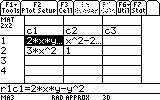
\includegraphics[width=.5\textwidth]{img/2NEWTON3.PNG}
\end{figure}

\begin{figure}[H]
	\centering
	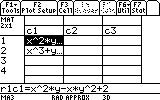
\includegraphics[width=.5\textwidth]{img/2NEWTON4.PNG}
\end{figure}

\pagebreak

Nyní spočítáme 1. aproximaci:

Do obou matic dosadíme počáteční aproximaci. Vektor f potřebujeme záporný:

\begin{figure}[H]
	\centering
	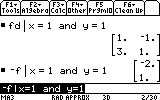
\includegraphics[width=.5\textwidth]{img/2NEWTON5.PNG}
\end{figure}

Nyní jsme schopni spočítat $\boldsymbol{\delta}^{(1)}$. Běžný způsob řešení soustavy lineárních rovnic by zde byl příliš zdlouhavý, proto využijeme podobný postup, jako při řešení MUN/MSP v předmětu EL1 a využijeme následujícího faktu:

\[
	\boldsymbol{\delta}^{(k)} = \mathbf{F'}(\mathbf{x}^{(k)})^{-1} \cdot \left( - \mathbf{F}(\mathbf{x}^{(k)}) \right)
\]

Dosazené matice můžeme do vstupního řádku zkopírovat stejným způsobem, jakým kopírujeme buňky v CellSheet. Spočtení $\boldsymbol{\delta}^{(1)}$ je pak triviální:

\begin{figure}[H]
	\centering
	\includegraphics[width=.5\textwidth]{img/2NEWTON6.PNG}
\end{figure}

\textit{Velmi zjednodušeně řečeno: zkopírujte dosazenou matici (tj. s čísly) do vstupního (dolního) řádku, dopište $\wedge$-1~*\\
Následně zkopírujte dosazenou f matici, vložte do vstupního řádku a stistkněte Enter.}

Abyste získali první aproximaci, musíte přičíst k výsledku $\boldsymbol{\delta}^{(0)}$, tedy počáteční aproximaci. Nejrychlejši bude vložit ji ručně jako matici přímo do vstupního řádku jako [[1][1]]. Tím získáte výslednou 1. aproximaci:

\begin{figure}[H]
	\centering
	\includegraphics[width=.5\textwidth]{img/2NEWTON7.PNG}
\end{figure}

\pagebreak

Podobným způsobem provedeme 2. aproximaci:

Do matice fd a -f dosadíme 1. aproximaci:

\begin{figure}[H]
	\centering
	\includegraphics[width=.5\textwidth]{img/2NEWTON8.PNG}
\end{figure}

Stejným způsobem jako v předchozím kroku spočítáme $\boldsymbol{\delta}^{(2)}$:

\begin{figure}[H]
	\centering
	\includegraphics[width=.5\textwidth]{img/2NEWTON9.PNG}
\end{figure}

Abychom získali výslednou 2. aproximaci, přičteme výsledek předchozího kroku:

\begin{figure}[H]
	\centering
	\includegraphics[width=.5\textwidth]{img/2NEWTON10.PNG}
\end{figure}

Tím jsme získali požadovaný výsledek.

\end{document}